% This example is meant to be compiled with lualatex or xelatex
% The theme itself also supports pdflatex
\PassOptionsToPackage{unicode}{hyperref}
\documentclass[aspectratio=1610, 12pt, xcolor=dvipsnames]{beamer}

% Warning, if another latex run is needed
% \usepackage[aux]{rerunfilecheck}

% just list chapters and sections in the toc, not subsections or smaller
\setcounter{tocdepth}{1}

%------------------------------------------------------------------------------
%------------------------------ Fonts, Unicode, Language ----------------------
%------------------------------------------------------------------------------
\usepackage{fontspec}
\defaultfontfeatures{Ligatures=TeX}  % -- becomes en-dash etc.

% german language
\usepackage{polyglossia}
\setdefaultlanguage{german}

% for english abstract and english titles in the toc
\setotherlanguages{english}

% intelligent quotation marks, language and nesting sensitive
\usepackage[autostyle]{csquotes}

% microtypographical features, makes the text look nicer on the small scale
\usepackage{microtype}

% colors and stuff
\usepackage{xcolor}
\usepackage[most]{tcolorbox}
\tcbset{on line, hbox,
        boxsep=4pt, left=0pt,right=0pt,top=0pt,bottom=0pt,
        colframe=white,colback=SpringGreen,
        highlight math style={enhanced}
        }
\newtcolorbox{mybox}[3][]
{
  colframe = #2!25,
  colback = #2!20,
  coltitle = #2!20!black,
  title = {#3},
  #1
}
%\colorlet{Green!40}
%------------------------------------------------------------------------------
%------------------------ Math Packages and settings --------------------------
%------------------------------------------------------------------------------

\usepackage{amsmath}
\usepackage{amssymb}
\usepackage{mathtools}
\usepackage{bbold}
\usepackage{hyperref}

% Enable Unicode-Math and follow the ISO-Standards for typesetting math
\usepackage[
  math-style=ISO,
  bold-style=ISO,
  sans-style=italic,
  nabla=upright,
  partial=upright,
]{unicode-math}
\setmathfont{Latin Modern Math}

% nice, small fracs for the text with \sfrac{}{}
\usepackage{xfrac}


%------------------------------------------------------------------------------
%---------------------------- Numbers and Units -------------------------------
%------------------------------------------------------------------------------

\usepackage[
  locale=DE,
  separate-uncertainty=true,
  per-mode=symbol-or-fraction,
]{siunitx}
\sisetup{math-micro=\text{µ},text-micro=µ}
% \sisetup{tophrase={{ to }}}
%------------------------------------------------------------------------------
%-------------------------------- tables  -------------------------------------
%------------------------------------------------------------------------------

\usepackage{booktabs}       % \toprule, \midrule, \bottomrule, etc

%------------------------------------------------------------------------------
%-------------------------------- graphics -------------------------------------
%------------------------------------------------------------------------------

\usepackage{graphicx}
%\usepackage{rotating}
\usepackage{grffile}
\usepackage{tikz}
\usepackage{circuitikz}
\usepackage{tikz-feynman}
\usepackage{subcaption}

% allow figures to be placed in the running text by default:
\usepackage{scrhack}
\usepackage{float}
\floatplacement{figure}{htbp}
\floatplacement{table}{htbp}

% keep figures and tables in the section
\usepackage[section, below]{placeins}

% smileys
\usepackage{MnSymbol,wasysym}

%------------------------------------------------------------------------------
%---------------------- customize list environments ---------------------------
%------------------------------------------------------------------------------

\usepackage{enumitem}
\usepackage{listings}
\usepackage{hepunits}

\usepackage{pdfpages}
%------------------------------------------------------------------------------
%------------------------------ Bibliographie ---------------------------------
%------------------------------------------------------------------------------

\usepackage[
  backend=biber,   % use modern biber backend
  autolang=hyphen, % load hyphenation rules for if language of bibentry is not
                   % german, has to be loaded with \setotherlanguages
                   % in the references.bib use langid={en} for english sources
]{biblatex}
\addbibresource{references.bib}  % the bib file to use
\DefineBibliographyStrings{german}{andothers = {{et\,al\adddot}}}  % replace u.a. with et al.


% Load packages you need here
% \usepackage{polyglossia}
% \setmainlanguage{german}

\usepackage{csquotes}


% \usepackage{amsmath}
% \usepackage{amssymb}
% \usepackage{mathtools}

\usepackage{hyperref}
\usepackage{bookmark}

% load the theme after all packages

\usetheme[
  showtotalframes, % show total number of frames in the footline
]{tudo}

% Put settings here, like
\unimathsetup{
  math-style=ISO,
  bold-style=ISO,
  nabla=upright,
  partial=upright,
  mathrm=sym,
}

% \setbeamertemplate{itemize item}{\scriptsize$\blacktriangleright$}
% \setbeamertemplate{itemize subitem}{\scriptsize$\blacktriangleright$}

%Titel:
\title{Global alignment of the LHCb SciFi Tracker and Vertex Locator}
%Autor
\author[N.Breer]{\textbf{Nils Breer}, Biljana Mitreska, Sophie Hollitt, Johannes Albrecht}
%Lehrstuhl/Fakultät
\institute{DPG Conference, Karlsruhe}
%Titelgrafik muss ich einfueren!!!
%\titlegraphic{\includegraphics[width=0.3\textwidth]{content/Bilder/interferenz.jpg}}
\date{04.03.2024}

\begin{document}
\maketitle

\begin{frame}\frametitle{Why do we need detector alignment?}
  \begin{columns}
    \begin{column}[c]{0.5\textwidth}
      \input{detector.tex}
    \end{column}
    \begin{column}[c]{0.5\textwidth}
      \begin{itemize}
        \item $\bullet$\, Track reconstruction accurately requires positions in reconstruction to be as similar as possible to real positions
        \item $\bullet$\, Top: ideal detector, bottom: physical detector
        \item $\bullet$\, Surveys are used to find the rotation and position of each detector component
        \item $\bullet$\, Input for alignment are surveyed measurements of detector positions
        \item $\bullet$\, Alignment goal: achieve the best precision in the detector position
      \end{itemize}
    \end{column}
  \end{columns}
\end{frame}

\begin{frame}\frametitle{Importance of alignments}
  \begin{itemize}
    \item $\bullet$\, Alignment is part of the LHCb trigger system
    \item $\bullet$\, Physics performance tied to alignment performance
    \item $\bullet$\, Good quality alignment contributes to:
    \begin{itemize}
      \item $\bullet$\, \to\, remove systematic biases for asymmetry measurements
      \item $\bullet$\, Best possible mass resolution
    \end{itemize}
  \end{itemize}
  % note: say in the talk: the alignment takes input from events selected by HLT1 to perform the calibration. the updated geometry constants are then applied both to HLT1 and HLT2
  \begin{figure}
      \includegraphics[width=0.9\textwidth]{logos/dataflow.png}%
    % \caption{Hits on tracks in x-direction with run 256145 data on 20000 ents using 9 minimum hits against 11 minimum hits.}
  \end{figure}
\end{frame}

\begin{frame}\frametitle{Tracking alignment: track fit using Kalman filter}
  \begin{columns}
    \begin{column}[c]{0.4\textwidth}
      \begin{figure}
        \centering
        \includegraphics[width=0.72\textwidth]{logos/kalman.png}
        % \caption{Alignment with Kalman Filter.}
      \end{figure}
    \end{column}
    \begin{column}[c]{0.55\textwidth}
      \begin{itemize}
        \item $\bullet$\, Starting positions: positions from laser scans of detector objects (survey)
        \item $\bullet$\, Alignment: $\chi^2$ minimization of track residuals
        \item $\bullet$\,\begin{equation}
          \frac{\symup{d}\Chi^2}{\symup{d}\alpha} = 2 A^T V^{-1}r
      \end{equation}
        \item $\bullet$\, Add measurements one-by-one to fit
        \item $\bullet$\, Prediction of next measurement \to minimize residuals \to redo until track complete
        \item $\bullet$\, Why Kalman Filter?
        \begin{itemize}
          \item $\bullet$\, Easily models material interactions as well as multiple scattering
        \end{itemize}
      \end{itemize}
    \end{column}
  \end{columns}
  % See \hyperfootnote[Kalman Filter]{https://www.sciencedirect.com/science/article/pii/S0168900208017567?via%3Dihub}
\end{frame}

\begin{frame}\frametitle{The Run 3 LHCb detector}
  \begin{columns}
    \begin{column}[c]{0.6\textwidth}
      \begin{figure}
        % \includegraphics[width=\textwidth]{logos/upgrade_lhcb.png}
        \includegraphics[width=\textwidth]{plots/lhcb_upgrade.png}
        % \caption{Visualization of the SciFi tracking stations.}
      \end{figure}
    \end{column}
    \begin{column}{0.48\textwidth}
      % \begin{itemize}
      %   \item $\bullet$\, 3 stations: T1, T2, T3
      %   \item $\bullet$\, 4 layers per station: X1, U, V, X2
      % 	\item $\bullet$\, Replaces former IT and OT to cope with the increased instantaneous luminosity
      %   \item $\bullet$\, IT and OT: silicon detectors have been replaced with fibre tracker
      % \end{itemize}
      \begin{itemize}
        \item $\bullet$\, Brand new detector to maintain physics performance at more radiation harsh environment
        \item $\bullet$\, UT was not present during 2022-23 data taking \to focus on SciFi and VELO
      \end{itemize}
      \begin{figure}
        \centering
        \includegraphics[width=\textwidth]{track.png}
      \end{figure}
    \end{column}
  \end{columns}
\end{frame}

\begin{frame}\frametitle{The Scintillating Fibre Tracker}
  \begin{columns}
    \begin{column}[c]{0.48\textwidth}
      \begin{figure}
        \includegraphics[width=0.9\textwidth]{logos/scifi.png}
        % \caption{Visualization of the SciFi tracking stations.}
      \end{figure}
    \end{column}
    \begin{column}{0.48\textwidth}
      \begin{itemize}
        \item $\bullet$\, 5 modules per side except for back T-station has 6
        \item $\bullet$\, X1, X2-layers are vertical and only yield x-position information
        \item $\bullet$\, U, V layers have a $\mp 5 \si{degree}$ stereo angle respectively
        \begin{itemize}
          \item $\bullet$\, \to\, Used for determining y-position of tracks by comparing hitposition at different angles
        \end{itemize}
      \end{itemize}
    \end{column}
  \end{columns}
\end{frame}

\begin{frame}\frametitle{VELO geometry}
  \begin{columns}
    \begin{column}[c]{0.5\textwidth}
      \begin{itemize}
        \item $\bullet$\, Rotation Rz leading to shifts in x and y
        % \item half alignment somewhat sensitive and shows Rz ≈ 3 mrad
        \item $\bullet$\, Half alignment sensitive to x shift
        \item $\bullet$\, Global movement in y
        \item $\bullet$\, Can not be corrected for by half alignment
      \end{itemize}    
    \end{column}
    \begin{column}[c]{0.5\textwidth}
      \begin{figure}
        \centering
        \includegraphics[width=\textwidth]{plots/velo_layers_all.png}
      \end{figure}
    \end{column}
  \end{columns}
  \includegraphics[width=\textwidth]{plots/velo_rotation.png}
\end{frame}

\begin{frame}\frametitle{Alignables for the global alignment}
  \begin{columns}
    \begin{column}[c]{0.5\textwidth}
      \begin{figure}
        \centering
        \includegraphics[width=0.9\textwidth]{plots/velo_halves.png}
      \end{figure}
    \end{column}
    \begin{column}{0.5\textwidth}
      \begin{figure}
        \centering
        \includegraphics[width=0.9\textwidth]{plots/scifi_modell.png}
      \end{figure}
    \end{column}
  \end{columns}
\end{frame}

\begin{frame}\frametitle{VELO ALignment}
  \begin{columns}
    \begin{column}[c]{0.5\textwidth}
      \begin{figure}
        \includegraphics[width=0.7\textwidth]{plots/velo_tracks_before_after.png}
        \includegraphics[width=0.7\textwidth]{plots/velo_deltax.png}
      \end{figure}
    \end{column}
    \begin{column}{0.5\textwidth}
      \begin{itemize}
        \item $\bullet$\, Align VELO in Tx to move modules where track is expected
      \end{itemize}
      \begin{figure}
        \centering
        \includegraphics[width=0.9\textwidth]{plots/PVx_velo.png}
      \end{figure}
    \end{column}
  \end{columns}
\end{frame}

\begin{frame}\frametitle{Global alignment and motivation}
  \begin{mybox}{green}{Global alignment}
    \begin{itemize}
      \item $\bullet$\, Alignment of the VELO and SciFi simultaneously
    \end{itemize}
    \begin{itemize}
      \setlength\itemsep{0em}
      \item $\bullet$\, Motivation for global alignment
      \begin{itemize}
        \item $\bullet$\, we can do the alignment seperately but ideally best alignment we achieve is the global one
        \item $\bullet$\, Understanding the interplay between tracking systems
        \item $\bullet$\, Rotations inside the VELO \to weak modes inside SciFi (VELO twisting)
      \end{itemize}
    \end{itemize}
  \end{mybox}
\end{frame}

\begin{frame}\frametitle{SciFi alignment status and issues}
  \begin{columns}
    \begin{column}[c]{0.6\textwidth}
      \begin{figure}
        \centering
        \includegraphics[width=0.9\textwidth]{plots/outfiles_vs_global/Layers_Tx_pattern.png}
      \end{figure}
    \end{column}
    \begin{column}[c]{0.4\textwidth}
      \begin{itemize}
        \item $\bullet$\, SciFi alignment is quite good already but there are some underlying problems
        \item $\bullet$\, Shift of SciFi layers larger than expected from survey
        \item $\bullet$\, Zig-zag pattern comes from global VELO Rx rotation
        \item $\bullet$\, Similar pattern in SciFi Tz \to entangled problem between Tx and Tz
      \end{itemize}
    \end{column}
  \end{columns}
\end{frame}

\begin{frame}\frametitle{Comparison to global alignment tests}
  \begin{table}
    \begin{tabular}{c | c c c c}
      \toprule
         & C-FRames & Halfmodules & full VELO & VELO halves \\
      \midrule
        DoF & RxRz & TxRxRz & RxRz & TxTyTz \\
      \bottomrule
    \end{tabular}
  \end{table}
  \begin{columns}
    \begin{column}[c]{0.48\textwidth}
      \begin{figure}
        \centering
        \includegraphics[width=\textwidth]{plots/outfiles_vs_global/all_runs_fix_glob_z_vs_local_Rz.pdf}
      \end{figure}
    \end{column}
    \begin{column}[c]{0.48\textwidth}
      \begin{itemize}
        \item $\bullet$\, Black: first align Longmodules then Halfmodules
        \item $\bullet$\, \color{blue}Blue\color{black}: constraining (X1|X2) and (U|V) layers
        \item $\bullet$\, \color{red}Red\color{black}: added backwards VELO tracks
        \item $\bullet$\, \color{green}Green\color{black}: only Rx in full VELO alignment
      \end{itemize}
    \end{column}
  \end{columns}
\end{frame}

\begin{frame}\frametitle{global alignment: rotation studies}
  \begin{columns}
    \begin{column}[c]{0.48\textwidth}
      \begin{figure}
        \centering
        \includegraphics[width=\textwidth]{plots/outfiles_vs_global/all_runs_fix_glob_z_vs_local_Rx.pdf}
      \end{figure}
    \end{column}
    \begin{column}[c]{0.48\textwidth}
      \begin{itemize}
        \item $\bullet$\, Observe rotation around Rx through T-stations \to inconsistent bending of the layers
        \item $\bullet$\, This effect only shows when running SciFi and VELO together
      \end{itemize}
    \end{column}
  \end{columns}
\end{frame}

\begin{frame}\frametitle{Outcome of the study and next steps}
  \begin{itemize}
    \setlength\itemsep{0em}
    \item $\bullet$\, ongoing investigation of zig-zag pattern with VELO Rx
    \item \to similar pattern in Tz \to cannot fix one without the other
    \item $\bullet$\, global VELO Rx might be overthrown by survey constrains acting on Rx \to Rx not being picked up in the alignment
    \item $\bullet$\, Testing different survey uncertanties to study the impact on global VELO rotation
    \item $\bullet$\, Testing different settings in the alignment on stereo layers in Tx
    \item $\bullet$\, make sure VELO Rx is being picked up in the alignment
    \item $\bullet$\, Include the VELO+ SciFi configuration during data-takin
  \end{itemize}
\end{frame}


\begin{frame}\frametitle{Summary}
  \begin{itemize}
    \setlength\itemsep{0em}
    \item $\bullet$\, global alignment improving the position of the T-stations
    \item $\bullet$\, survey constraints might counteract the global VELO Rx
    \item $\bullet$\, A lot more tests to do until data taking which look promising
    \item $\bullet$\, \textbf{Thank you for your attention!}
  \end{itemize}
  % \textbf{Thank you for your attention!}
\end{frame}

% \begin{frame}\frametitle{Backup: SciFi terminology}
%   Layers are divided into two halves commonly labeled as A-side and C-side
%   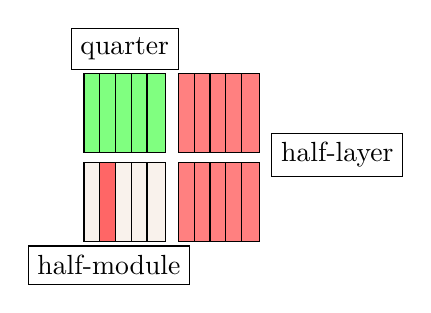
\begin{tikzpicture}
% first quarter
  \node[rectangle,
      draw = black,
      % text = ,
      fill = brown!10!white,
      minimum width = 0.2cm,
      minimum height = 1cm] (r) at (0,0) {};

  \node[rectangle,
      draw = black,
      % text = half-module,
      fill = red!60!white,
      minimum width = 0.2cm,
      minimum height = 1cm] (r) at (0.2,0) {};

  \node[rectangle,
      draw = black,
      % text = ,
      fill = brown!10!white,
      minimum width = 0.2cm,
      minimum height = 1cm] (r) at (0.4,0) {};

  \node[rectangle,
      draw = black,
      % text = ,
      fill = brown!10!white,
      minimum width = 0.2cm,
      minimum height = 1cm] (r) at (0.6,0) {};

  \node[rectangle,
      draw = black,
      % text = ,
      fill = brown!10!white,
      minimum width = 0.2cm,
      minimum height = 1cm] (r) at (0.8,0) {};

% second quarter
\node[rectangle,
    draw = black,
    % text = ,
    fill = red!50!white,
    minimum width = 0.2cm,
    minimum height = 1cm] (r) at (1.2,0) {};

\node[rectangle,
    draw = black,
    % text = ,
    fill = red!50!white,
    minimum width = 0.2cm,
    minimum height = 1cm] (r) at (1.4,0) {};

\node[rectangle,
    draw = black,
    % text = ,
    fill = red!50!white,
    minimum width = 0.2cm,
    minimum height = 1cm] (r) at (1.6,0) {};

\node[rectangle,
    draw = black,
    % text = ,
    fill = red!50!white,
    minimum width = 0.2cm,
    minimum height = 1cm] (r) at (1.8,0) {};

\node[rectangle,
    draw = black,
    % text = ,
    fill = red!50!white,
    minimum width = 0.2cm,
    minimum height = 1cm] (r) at (2,0) {};

% third quarter
\node[rectangle,
    draw = black,
    % text = ,
    fill = green!50!white,
    minimum width = 0.2cm,
    minimum height = 1cm] (r) at (0,1.13) {};

\node[rectangle,
    draw = black,
    % text = quarter,
    fill = green!50!white,
    minimum width = 0.2cm,
    minimum height = 1cm] (r) at (0.2,1.13) {};

\node[rectangle,
    draw = black,
    % text = ,
    fill = green!50!white,
    minimum width = 0.2cm,
    minimum height = 1cm] (r) at (0.4,1.13) {};

\node[rectangle,
    draw = black,
    % text = ,
    fill = green!50!white,
    minimum width = 0.2cm,
    minimum height = 1cm] (r) at (0.6,1.13) {};

\node[rectangle,
    draw = black,
    % text = ,
    fill = green!50!white,
    minimum width = 0.2cm,
    minimum height = 1cm] (r) at (0.8,1.13) {};

% fourth quarter
\node[rectangle,
    draw = black,
    % text = ,
    fill = red!50!white,
    minimum width = 0.2cm,
    minimum height = 1cm] (r) at (1.2,1.13) {};

\node[rectangle,
    draw = black,
    % text = ,
    fill = red!50!white,
    minimum width = 0.2cm,
    minimum height = 1cm] (r) at (1.4,1.13) {};

\node[rectangle,
    draw = black,
    % text = ,
    fill = red!50!white,
    minimum width = 0.2cm,
    minimum height = 1cm] (r) at (1.6,1.13) {};

\node[rectangle,
    draw = black,
    % text = ,
    fill = red!50!white,
    minimum width = 0.2cm,
    minimum height = 1cm] (r) at (1.8,1.13) {};

\node[rectangle,
    draw = black,
    % text = ,
    fill = red!50!white,
    minimum width = 0.2cm,
    minimum height = 1cm] (r) at (2,1.13) {};

\node[draw] at (0.4, 1.95) {quarter};
\node[draw] at (0.2, -0.8) {half-module};
\node[draw] at (3.1, 0.6) {half-layer};

\end{tikzpicture}

% \end{frame}

\begin{frame}\frametitle{The survey: what is it and the different types}
  \begin{columns}
    \begin{column}[c]{0.48\textwidth}
      $\bullet$\, Measure distance of some points on the detector with a laser
      \begin{figure}
        \centering
        \includegraphics[width=\textwidth]{logos/survey.png}
        % \caption{}
      \end{figure}
    \end{column}
    \begin{column}[c]{0.48\textwidth}
      \begin{itemize}
        \item $\bullet$\, Layer survey: find corners of layers
        \item $\bullet$\, Module survey: reflective stickers, calculate module plane
        \item $\bullet$\, Compare survey to simulation
      \end{itemize}
    \end{column}
  \end{columns}
\end{frame}

% \begin{frame}
%   \begin{figure}
%     \includegraphics[width=\textwidth]{plots/old_lhcb.png}
%   \end{figure}
% \end{frame}


% not needed
% \begin{frame}\frametitle{Sources}
%   \begin{itemize}
%     \item $\bullet$\,SciFi Conference Talk: \url{https://twiki.cern.ch/twiki/pub/LHCb/SciFiConference/fee_2018.pdf}
%     \item $\bullet$\,LHCb SciFi: From performance requirements to an operational detector: \url{https://indico.cern.ch/event/1163878/}
%     \item $\bullet$\, BCAM \url{https://accelconf.web.cern.ch/ipac2018/papers/wepaf067.pdf}
%   \end{itemize}
% \end{frame}

\end{document}
